\begin{tikzpicture}[scale=.2, anchor=south west]
\node[draw=black, rectangle split, rectangle split parts=3] (sn0x8d72c50W-4) at (-4.75, -15) {
\begin{tikzpicture}[scale=.2]
\node[circle, scale=0.75, fill] (tid0) at (3.75,0){};
\node[circle, scale=0.75, fill] (tid1) at (2.25,1.5){};
\node[circle, scale=0.75, fill] (tid3) at (0.75,3){};
\node[circle, scale=0.75, fill, red] (tid8) at (0.75,4.5){};
\draw[](tid3) -- (tid8);
\node[circle, scale=0.75, fill, red] (tid4) at (2.25,3){};
\node[circle, scale=0.75, fill] (tid5) at (3.75,3){};
\draw[](tid1) -- (tid3);
\draw[](tid1) -- (tid4);
\draw[](tid1) -- (tid5);
\node[circle, scale=0.75, fill] (tid2) at (6,1.5){};
\node[circle, scale=0.75, fill, red] (tid6) at (5.25,3){};
\node[circle, scale=0.75, fill] (tid7) at (6.75,3){};
\draw[](tid2) -- (tid6);
\draw[](tid2) -- (tid7);
\draw[](tid0) -- (tid1);
\draw[](tid0) -- (tid2);

\end{tikzpicture}
\nodepart{two}
\footnotesize{5.15072}
\nodepart{three}
\footnotesize{$17\:17\:17\:17\:22\:11$}
};
\node[draw=black, rectangle split, rectangle split parts=3] (sn0x8d75c30W-25) at (-25.5, -30) {
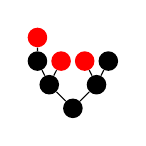
\begin{tikzpicture}[scale=.2]
\node[circle, scale=0.75, fill] (tid0) at (3,0){};
\node[circle, scale=0.75, fill] (tid1) at (1.5,1.5){};
\node[circle, scale=0.75, fill] (tid3) at (0.75,3){};
\node[circle, scale=0.75, fill, red] (tid7) at (0.75,4.5){};
\draw[](tid3) -- (tid7);
\node[circle, scale=0.75, fill, red] (tid4) at (2.25,3){};
\draw[](tid1) -- (tid3);
\draw[](tid1) -- (tid4);
\node[circle, scale=0.75, fill] (tid2) at (4.5,1.5){};
\node[circle, scale=0.75, fill, red] (tid5) at (3.75,3){};
\node[circle, scale=0.75, fill] (tid6) at (5.25,3){};
\draw[](tid2) -- (tid5);
\draw[](tid2) -- (tid6);
\draw[](tid0) -- (tid1);
\draw[](tid0) -- (tid2);

\end{tikzpicture}
\nodepart{two}
\footnotesize{4.88195}
\nodepart{three}
\footnotesize{$33\:33\:33$}
};
\node[draw=black, rectangle split, rectangle split parts=3] (sn0x8d767d0W-22) at (-22.5, -45) {
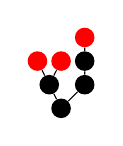
\begin{tikzpicture}[scale=.2]
\node[circle, scale=0.75, fill] (tid0) at (2.25,0){};
\node[circle, scale=0.75, fill] (tid1) at (1.5,1.5){};
\node[circle, scale=0.75, fill, red] (tid3) at (0.75,3){};
\node[circle, scale=0.75, fill, red] (tid4) at (2.25,3){};
\draw[](tid1) -- (tid3);
\draw[](tid1) -- (tid4);
\node[circle, scale=0.75, fill] (tid2) at (3.75,1.5){};
\node[circle, scale=0.75, fill] (tid5) at (3.75,3){};
\node[circle, scale=0.75, fill, red] (tid6) at (3.75,4.5){};
\draw[](tid5) -- (tid6);
\draw[](tid2) -- (tid5);
\draw[](tid0) -- (tid1);
\draw[](tid0) -- (tid2);

\end{tikzpicture}
\nodepart{two}
\footnotesize{4.64352}
\nodepart{three}
\footnotesize{$67\:33$}
};
\node[draw=black, rectangle split, rectangle split parts=3] (sn0x8d77318W-13) at (-13, -60) {
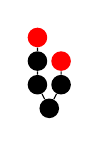
\begin{tikzpicture}[scale=.2]
\node[circle, scale=0.75, fill] (tid0) at (1.5,0){};
\node[circle, scale=0.75, fill] (tid1) at (0.75,1.5){};
\node[circle, scale=0.75, fill] (tid3) at (0.75,3){};
\node[circle, scale=0.75, fill, red] (tid5) at (0.75,4.5){};
\draw[](tid3) -- (tid5);
\draw[](tid1) -- (tid3);
\node[circle, scale=0.75, fill] (tid2) at (2.25,1.5){};
\node[circle, scale=0.75, fill, red] (tid4) at (2.25,3){};
\draw[](tid2) -- (tid4);
\draw[](tid0) -- (tid1);
\draw[](tid0) -- (tid2);

\end{tikzpicture}
\nodepart{two}
\footnotesize{4.4375}
\nodepart{three}
\footnotesize{$50\:50$}
};
\node[draw=black, rectangle split, rectangle split parts=3] (sn0x8d77448W-10) at (-10.75, -75) {
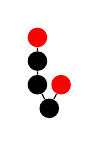
\begin{tikzpicture}[scale=.2]
\node[circle, scale=0.75, fill] (tid0) at (1.5,0){};
\node[circle, scale=0.75, fill] (tid1) at (0.75,1.5){};
\node[circle, scale=0.75, fill] (tid3) at (0.75,3){};
\node[circle, scale=0.75, fill, red] (tid4) at (0.75,4.5){};
\draw[](tid3) -- (tid4);
\draw[](tid1) -- (tid3);
\node[circle, scale=0.75, fill, red] (tid2) at (2.25,1.5){};
\draw[](tid0) -- (tid1);
\draw[](tid0) -- (tid2);

\end{tikzpicture}
\nodepart{two}
\footnotesize{4.125}
\nodepart{three}
\footnotesize{$50\:50$}
};
\node[draw=black, rectangle split, rectangle split parts=3] (sn0x8d77658W-6) at (-6.75, -90) {
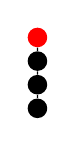
\begin{tikzpicture}[scale=.2]
\node[circle, scale=0.75, fill] (tid0) at (0.75,0){};
\node[circle, scale=0.75, fill] (tid1) at (0.75,1.5){};
\node[circle, scale=0.75, fill] (tid2) at (0.75,3){};
\node[circle, scale=0.75, fill, red] (tid3) at (0.75,4.5){};
\draw[](tid2) -- (tid3);
\draw[](tid1) -- (tid2);
\draw[](tid0) -- (tid1);

\end{tikzpicture}
\nodepart{two}
\footnotesize{4}
\nodepart{three}
\footnotesize{$1$}
};
\node[draw=black, rectangle split, rectangle split parts=3] (sn0x8d77980W-4) at (-4.25, -105) {
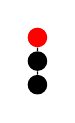
\begin{tikzpicture}[scale=.2]
\node[circle, scale=0.75, fill] (tid0) at (0.75,0){};
\node[circle, scale=0.75, fill] (tid1) at (0.75,1.5){};
\node[circle, scale=0.75, fill, red] (tid2) at (0.75,3){};
\draw[](tid1) -- (tid2);
\draw[](tid0) -- (tid1);

\end{tikzpicture}
\nodepart{two}
\footnotesize{3}
\nodepart{three}
\footnotesize{$1$}
};
\node[draw=black, rectangle split, rectangle split parts=3] (sn0x8d77af8W-1) at (-1.75, -120) {

\begin{tikzpicture}[scale=.2]
\node[circle, scale=0.75, fill] (tid0) at (0.75,0){};
\node[circle, scale=0.75, fill, red] (tid1) at (0.75,1.5){};
\draw[](tid0) -- (tid1);

\end{tikzpicture}
\nodepart{two}
\footnotesize{2}
\nodepart{three}
\footnotesize{$1$}
};
\draw (sn0x8d77980W-4.south) -- (sn0x8d77af8W-1.north);
\draw (sn0x8d77658W-6.south) -- (sn0x8d77980W-4.north);
\node[draw=black, rectangle split, rectangle split parts=3] (sn0x8d77810W-3) at (-3.25, -90) {
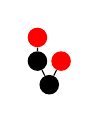
\begin{tikzpicture}[scale=.2]
\node[circle, scale=0.75, fill] (tid0) at (1.5,0){};
\node[circle, scale=0.75, fill] (tid1) at (0.75,1.5){};
\node[circle, scale=0.75, fill, red] (tid3) at (0.75,3){};
\draw[](tid1) -- (tid3);
\node[circle, scale=0.75, fill, red] (tid2) at (2.25,1.5){};
\draw[](tid0) -- (tid1);
\draw[](tid0) -- (tid2);

\end{tikzpicture}
\nodepart{two}
\footnotesize{3.25}
\nodepart{three}
\footnotesize{$50\:50$}
};
\node[draw=black, rectangle split, rectangle split parts=3] (sn0x8d77cb8W0) at (-0.75, -105) {

\begin{tikzpicture}[scale=.2]
\node[circle, scale=0.75, fill] (tid0) at (1.5,0){};
\node[circle, scale=0.75, fill, red] (tid1) at (0.75,1.5){};
\node[circle, scale=0.75, fill, red] (tid2) at (2.25,1.5){};
\draw[](tid0) -- (tid1);
\draw[](tid0) -- (tid2);

\end{tikzpicture}
\nodepart{two}
\footnotesize{2.5}
\nodepart{three}
\footnotesize{$1$}
};
\draw (sn0x8d77cb8W0.south) -- (sn0x8d77af8W-1.north);
\draw (sn0x8d77810W-3.south) -- (sn0x8d77980W-4.north);
\draw (sn0x8d77810W-3.south) -- (sn0x8d77cb8W0.north);
\draw (sn0x8d77448W-10.south) -- (sn0x8d77658W-6.north);
\draw (sn0x8d77448W-10.south) -- (sn0x8d77810W-3.north);
\node[draw=black, rectangle split, rectangle split parts=3] (sn0x8d775f0W-5) at (-5.75, -75) {
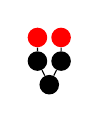
\begin{tikzpicture}[scale=.2]
\node[circle, scale=0.75, fill] (tid0) at (1.5,0){};
\node[circle, scale=0.75, fill] (tid1) at (0.75,1.5){};
\node[circle, scale=0.75, fill, red] (tid3) at (0.75,3){};
\draw[](tid1) -- (tid3);
\node[circle, scale=0.75, fill] (tid2) at (2.25,1.5){};
\node[circle, scale=0.75, fill, red] (tid4) at (2.25,3){};
\draw[](tid2) -- (tid4);
\draw[](tid0) -- (tid1);
\draw[](tid0) -- (tid2);

\end{tikzpicture}
\nodepart{two}
\footnotesize{3.75}
\nodepart{three}
\footnotesize{$1$}
};
\draw (sn0x8d775f0W-5.south) -- (sn0x8d77810W-3.north);
\draw (sn0x8d77318W-13.south) -- (sn0x8d77448W-10.north);
\draw (sn0x8d77318W-13.south) -- (sn0x8d775f0W-5.north);
\node[draw=black, rectangle split, rectangle split parts=3] (sn0x8d773b0W-8) at (-8, -60) {
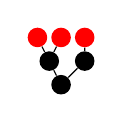
\begin{tikzpicture}[scale=.2]
\node[circle, scale=0.75, fill] (tid0) at (2.25,0){};
\node[circle, scale=0.75, fill] (tid1) at (1.5,1.5){};
\node[circle, scale=0.75, fill, red] (tid3) at (0.75,3){};
\node[circle, scale=0.75, fill, red] (tid4) at (2.25,3){};
\draw[](tid1) -- (tid3);
\draw[](tid1) -- (tid4);
\node[circle, scale=0.75, fill] (tid2) at (3.75,1.5){};
\node[circle, scale=0.75, fill, red] (tid5) at (3.75,3){};
\draw[](tid2) -- (tid5);
\draw[](tid0) -- (tid1);
\draw[](tid0) -- (tid2);

\end{tikzpicture}
\nodepart{two}
\footnotesize{4.05556}
\nodepart{three}
\footnotesize{$67\:33$}
};
\node[draw=black, rectangle split, rectangle split parts=3] (sn0x8d78058W0) at (-0.75, -75) {
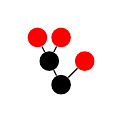
\begin{tikzpicture}[scale=.2]
\node[circle, scale=0.75, fill] (tid0) at (2.25,0){};
\node[circle, scale=0.75, fill] (tid1) at (1.5,1.5){};
\node[circle, scale=0.75, fill, red] (tid3) at (0.75,3){};
\node[circle, scale=0.75, fill, red] (tid4) at (2.25,3){};
\draw[](tid1) -- (tid3);
\draw[](tid1) -- (tid4);
\node[circle, scale=0.75, fill, red] (tid2) at (3.75,1.5){};
\draw[](tid0) -- (tid1);
\draw[](tid0) -- (tid2);

\end{tikzpicture}
\nodepart{two}
\footnotesize{3.66667}
\nodepart{three}
\footnotesize{$67\:33$}
};
\node[draw=black, rectangle split, rectangle split parts=3] (sn0x8d781a8W1) at (1.75, -90) {
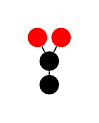
\begin{tikzpicture}[scale=.2]
\node[circle, scale=0.75, fill] (tid0) at (1.5,0){};
\node[circle, scale=0.75, fill] (tid1) at (1.5,1.5){};
\node[circle, scale=0.75, fill, red] (tid2) at (0.75,3){};
\node[circle, scale=0.75, fill, red] (tid3) at (2.25,3){};
\draw[](tid1) -- (tid2);
\draw[](tid1) -- (tid3);
\draw[](tid0) -- (tid1);

\end{tikzpicture}
\nodepart{two}
\footnotesize{3.5}
\nodepart{three}
\footnotesize{$1$}
};
\draw (sn0x8d781a8W1.south) -- (sn0x8d77980W-4.north);
\draw (sn0x8d78058W0.south) -- (sn0x8d781a8W1.north);
\draw (sn0x8d78058W0.south) -- (sn0x8d77810W-3.north);
\draw (sn0x8d773b0W-8.south) -- (sn0x8d775f0W-5.north);
\draw (sn0x8d773b0W-8.south) -- (sn0x8d78058W0.north);
\draw (sn0x8d767d0W-22.south) -- (sn0x8d77318W-13.north);
\draw (sn0x8d767d0W-22.south) -- (sn0x8d773b0W-8.north);
\node[draw=black, rectangle split, rectangle split parts=3] (sn0x8d76d60W-16) at (-16, -45) {
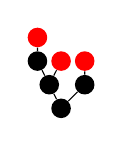
\begin{tikzpicture}[scale=.2]
\node[circle, scale=0.75, fill] (tid0) at (2.25,0){};
\node[circle, scale=0.75, fill] (tid1) at (1.5,1.5){};
\node[circle, scale=0.75, fill] (tid3) at (0.75,3){};
\node[circle, scale=0.75, fill, red] (tid6) at (0.75,4.5){};
\draw[](tid3) -- (tid6);
\node[circle, scale=0.75, fill, red] (tid4) at (2.25,3){};
\draw[](tid1) -- (tid3);
\draw[](tid1) -- (tid4);
\node[circle, scale=0.75, fill] (tid2) at (3.75,1.5){};
\node[circle, scale=0.75, fill, red] (tid5) at (3.75,3){};
\draw[](tid2) -- (tid5);
\draw[](tid0) -- (tid1);
\draw[](tid0) -- (tid2);

\end{tikzpicture}
\nodepart{two}
\footnotesize{4.61343}
\nodepart{three}
\footnotesize{$33\:33\:33$}
};
\node[draw=black, rectangle split, rectangle split parts=3] (sn0x8d78990W-1) at (-1.5, -60) {
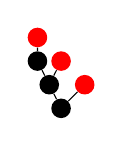
\begin{tikzpicture}[scale=.2]
\node[circle, scale=0.75, fill] (tid0) at (2.25,0){};
\node[circle, scale=0.75, fill] (tid1) at (1.5,1.5){};
\node[circle, scale=0.75, fill] (tid3) at (0.75,3){};
\node[circle, scale=0.75, fill, red] (tid5) at (0.75,4.5){};
\draw[](tid3) -- (tid5);
\node[circle, scale=0.75, fill, red] (tid4) at (2.25,3){};
\draw[](tid1) -- (tid3);
\draw[](tid1) -- (tid4);
\node[circle, scale=0.75, fill, red] (tid2) at (3.75,1.5){};
\draw[](tid0) -- (tid1);
\draw[](tid0) -- (tid2);

\end{tikzpicture}
\nodepart{two}
\footnotesize{4.34722}
\nodepart{three}
\footnotesize{$33\:33\:33$}
};
\node[draw=black, rectangle split, rectangle split parts=3] (sn0x8d78430W5) at (5.75, -75) {
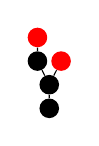
\begin{tikzpicture}[scale=.2]
\node[circle, scale=0.75, fill] (tid0) at (1.5,0){};
\node[circle, scale=0.75, fill] (tid1) at (1.5,1.5){};
\node[circle, scale=0.75, fill] (tid2) at (0.75,3){};
\node[circle, scale=0.75, fill, red] (tid4) at (0.75,4.5){};
\draw[](tid2) -- (tid4);
\node[circle, scale=0.75, fill, red] (tid3) at (2.25,3){};
\draw[](tid1) -- (tid2);
\draw[](tid1) -- (tid3);
\draw[](tid0) -- (tid1);

\end{tikzpicture}
\nodepart{two}
\footnotesize{4.25}
\nodepart{three}
\footnotesize{$50\:50$}
};
\draw (sn0x8d78430W5.south) -- (sn0x8d77658W-6.north);
\draw (sn0x8d78430W5.south) -- (sn0x8d781a8W1.north);
\draw (sn0x8d78990W-1.south) -- (sn0x8d78430W5.north);
\draw (sn0x8d78990W-1.south) -- (sn0x8d77448W-10.north);
\draw (sn0x8d78990W-1.south) -- (sn0x8d78058W0.north);
\draw (sn0x8d76d60W-16.south) -- (sn0x8d77318W-13.north);
\draw (sn0x8d76d60W-16.south) -- (sn0x8d78990W-1.north);
\draw (sn0x8d76d60W-16.south) -- (sn0x8d773b0W-8.north);
\node[draw=black, rectangle split, rectangle split parts=3] (sn0x8d76e58W-9) at (-9.5, -45) {
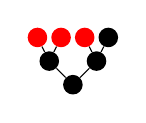
\begin{tikzpicture}[scale=.2]
\node[circle, scale=0.75, fill] (tid0) at (3,0){};
\node[circle, scale=0.75, fill] (tid1) at (1.5,1.5){};
\node[circle, scale=0.75, fill, red] (tid3) at (0.75,3){};
\node[circle, scale=0.75, fill, red] (tid4) at (2.25,3){};
\draw[](tid1) -- (tid3);
\draw[](tid1) -- (tid4);
\node[circle, scale=0.75, fill] (tid2) at (4.5,1.5){};
\node[circle, scale=0.75, fill, red] (tid5) at (3.75,3){};
\node[circle, scale=0.75, fill] (tid6) at (5.25,3){};
\draw[](tid2) -- (tid5);
\draw[](tid2) -- (tid6);
\draw[](tid0) -- (tid1);
\draw[](tid0) -- (tid2);

\end{tikzpicture}
\nodepart{two}
\footnotesize{4.38889}
\nodepart{three}
\footnotesize{$1$}
};
\draw (sn0x8d76e58W-9.south) -- (sn0x8d773b0W-8.north);
\draw (sn0x8d75c30W-25.south) -- (sn0x8d767d0W-22.north);
\draw (sn0x8d75c30W-25.south) -- (sn0x8d76d60W-16.north);
\draw (sn0x8d75c30W-25.south) -- (sn0x8d76e58W-9.north);
\node[draw=black, rectangle split, rectangle split parts=3] (sn0x8d75280W-17) at (-17.5, -30) {
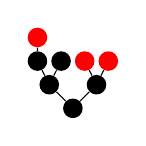
\begin{tikzpicture}[scale=.2]
\node[circle, scale=0.75, fill] (tid0) at (3,0){};
\node[circle, scale=0.75, fill] (tid1) at (1.5,1.5){};
\node[circle, scale=0.75, fill] (tid3) at (0.75,3){};
\node[circle, scale=0.75, fill, red] (tid7) at (0.75,4.5){};
\draw[](tid3) -- (tid7);
\node[circle, scale=0.75, fill] (tid4) at (2.25,3){};
\draw[](tid1) -- (tid3);
\draw[](tid1) -- (tid4);
\node[circle, scale=0.75, fill] (tid2) at (4.5,1.5){};
\node[circle, scale=0.75, fill, red] (tid5) at (3.75,3){};
\node[circle, scale=0.75, fill, red] (tid6) at (5.25,3){};
\draw[](tid2) -- (tid5);
\draw[](tid2) -- (tid6);
\draw[](tid0) -- (tid1);
\draw[](tid0) -- (tid2);

\end{tikzpicture}
\nodepart{two}
\footnotesize{4.87191}
\nodepart{three}
\footnotesize{$33\:67$}
};
\draw (sn0x8d75280W-17.south) -- (sn0x8d76d60W-16.north);
\draw (sn0x8d75280W-17.south) -- (sn0x8d76e58W-9.north);
\node[draw=black, rectangle split, rectangle split parts=3] (sn0x8d75918W-9) at (-9.5, -30) {
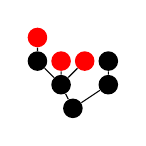
\begin{tikzpicture}[scale=.2]
\node[circle, scale=0.75, fill] (tid0) at (3,0){};
\node[circle, scale=0.75, fill] (tid1) at (2.25,1.5){};
\node[circle, scale=0.75, fill] (tid3) at (0.75,3){};
\node[circle, scale=0.75, fill, red] (tid7) at (0.75,4.5){};
\draw[](tid3) -- (tid7);
\node[circle, scale=0.75, fill, red] (tid4) at (2.25,3){};
\node[circle, scale=0.75, fill, red] (tid5) at (3.75,3){};
\draw[](tid1) -- (tid3);
\draw[](tid1) -- (tid4);
\draw[](tid1) -- (tid5);
\node[circle, scale=0.75, fill] (tid2) at (5.25,1.5){};
\node[circle, scale=0.75, fill] (tid6) at (5.25,3){};
\draw[](tid2) -- (tid6);
\draw[](tid0) -- (tid1);
\draw[](tid0) -- (tid2);

\end{tikzpicture}
\nodepart{two}
\footnotesize{4.86883}
\nodepart{three}
\footnotesize{$67\:17\:17$}
};
\node[draw=black, rectangle split, rectangle split parts=3] (sn0x8d78b18W-1) at (-1.5, -45) {
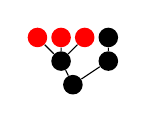
\begin{tikzpicture}[scale=.2]
\node[circle, scale=0.75, fill] (tid0) at (3,0){};
\node[circle, scale=0.75, fill] (tid1) at (2.25,1.5){};
\node[circle, scale=0.75, fill, red] (tid3) at (0.75,3){};
\node[circle, scale=0.75, fill, red] (tid4) at (2.25,3){};
\node[circle, scale=0.75, fill, red] (tid5) at (3.75,3){};
\draw[](tid1) -- (tid3);
\draw[](tid1) -- (tid4);
\draw[](tid1) -- (tid5);
\node[circle, scale=0.75, fill] (tid2) at (5.25,1.5){};
\node[circle, scale=0.75, fill] (tid6) at (5.25,3){};
\draw[](tid2) -- (tid6);
\draw[](tid0) -- (tid1);
\draw[](tid0) -- (tid2);

\end{tikzpicture}
\nodepart{two}
\footnotesize{4.38889}
\nodepart{three}
\footnotesize{$1$}
};
\draw (sn0x8d78b18W-1.south) -- (sn0x8d773b0W-8.north);
\node[draw=black, rectangle split, rectangle split parts=3] (sn0x8d78f78W6) at (6.5, -45) {
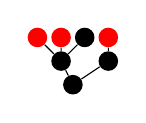
\begin{tikzpicture}[scale=.2]
\node[circle, scale=0.75, fill] (tid0) at (3,0){};
\node[circle, scale=0.75, fill] (tid1) at (2.25,1.5){};
\node[circle, scale=0.75, fill, red] (tid3) at (0.75,3){};
\node[circle, scale=0.75, fill, red] (tid4) at (2.25,3){};
\node[circle, scale=0.75, fill] (tid5) at (3.75,3){};
\draw[](tid1) -- (tid3);
\draw[](tid1) -- (tid4);
\draw[](tid1) -- (tid5);
\node[circle, scale=0.75, fill] (tid2) at (5.25,1.5){};
\node[circle, scale=0.75, fill, red] (tid6) at (5.25,3){};
\draw[](tid2) -- (tid6);
\draw[](tid0) -- (tid1);
\draw[](tid0) -- (tid2);

\end{tikzpicture}
\nodepart{two}
\footnotesize{4.37037}
\nodepart{three}
\footnotesize{$67\:33$}
};
\node[draw=black, rectangle split, rectangle split parts=3] (sn0x8d78a68W5) at (5, -60) {
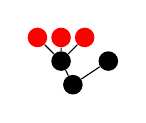
\begin{tikzpicture}[scale=.2]
\node[circle, scale=0.75, fill] (tid0) at (3,0){};
\node[circle, scale=0.75, fill] (tid1) at (2.25,1.5){};
\node[circle, scale=0.75, fill, red] (tid3) at (0.75,3){};
\node[circle, scale=0.75, fill, red] (tid4) at (2.25,3){};
\node[circle, scale=0.75, fill, red] (tid5) at (3.75,3){};
\draw[](tid1) -- (tid3);
\draw[](tid1) -- (tid4);
\draw[](tid1) -- (tid5);
\node[circle, scale=0.75, fill] (tid2) at (5.25,1.5){};
\draw[](tid0) -- (tid1);
\draw[](tid0) -- (tid2);

\end{tikzpicture}
\nodepart{two}
\footnotesize{4}
\nodepart{three}
\footnotesize{$1$}
};
\draw (sn0x8d78a68W5.south) -- (sn0x8d78058W0.north);
\draw (sn0x8d78f78W6.south) -- (sn0x8d773b0W-8.north);
\draw (sn0x8d78f78W6.south) -- (sn0x8d78a68W5.north);
\draw (sn0x8d75918W-9.south) -- (sn0x8d76d60W-16.north);
\draw (sn0x8d75918W-9.south) -- (sn0x8d78b18W-1.north);
\draw (sn0x8d75918W-9.south) -- (sn0x8d78f78W6.north);
\node[draw=black, rectangle split, rectangle split parts=3] (sn0x8d718a8W-1) at (-1.5, -30) {
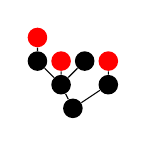
\begin{tikzpicture}[scale=.2]
\node[circle, scale=0.75, fill] (tid0) at (3,0){};
\node[circle, scale=0.75, fill] (tid1) at (2.25,1.5){};
\node[circle, scale=0.75, fill] (tid3) at (0.75,3){};
\node[circle, scale=0.75, fill, red] (tid7) at (0.75,4.5){};
\draw[](tid3) -- (tid7);
\node[circle, scale=0.75, fill, red] (tid4) at (2.25,3){};
\node[circle, scale=0.75, fill] (tid5) at (3.75,3){};
\draw[](tid1) -- (tid3);
\draw[](tid1) -- (tid4);
\draw[](tid1) -- (tid5);
\node[circle, scale=0.75, fill] (tid2) at (5.25,1.5){};
\node[circle, scale=0.75, fill, red] (tid6) at (5.25,3){};
\draw[](tid2) -- (tid6);
\draw[](tid0) -- (tid1);
\draw[](tid0) -- (tid2);

\end{tikzpicture}
\nodepart{two}
\footnotesize{4.84954}
\nodepart{three}
\footnotesize{$33\:33\:33$}
};
\node[draw=black, rectangle split, rectangle split parts=3] (sn0x8d791d0W14) at (14.5, -45) {
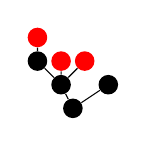
\begin{tikzpicture}[scale=.2]
\node[circle, scale=0.75, fill] (tid0) at (3,0){};
\node[circle, scale=0.75, fill] (tid1) at (2.25,1.5){};
\node[circle, scale=0.75, fill] (tid3) at (0.75,3){};
\node[circle, scale=0.75, fill, red] (tid6) at (0.75,4.5){};
\draw[](tid3) -- (tid6);
\node[circle, scale=0.75, fill, red] (tid4) at (2.25,3){};
\node[circle, scale=0.75, fill, red] (tid5) at (3.75,3){};
\draw[](tid1) -- (tid3);
\draw[](tid1) -- (tid4);
\draw[](tid1) -- (tid5);
\node[circle, scale=0.75, fill] (tid2) at (5.25,1.5){};
\draw[](tid0) -- (tid1);
\draw[](tid0) -- (tid2);

\end{tikzpicture}
\nodepart{two}
\footnotesize{4.56482}
\nodepart{three}
\footnotesize{$33\:67$}
};
\draw (sn0x8d791d0W14.south) -- (sn0x8d78990W-1.north);
\draw (sn0x8d791d0W14.south) -- (sn0x8d78a68W5.north);
\draw (sn0x8d718a8W-1.south) -- (sn0x8d76d60W-16.north);
\draw (sn0x8d718a8W-1.south) -- (sn0x8d791d0W14.north);
\draw (sn0x8d718a8W-1.south) -- (sn0x8d78f78W6.north);
\node[draw=black, rectangle split, rectangle split parts=3] (sn0x8d75fb0W6) at (6.5, -30) {
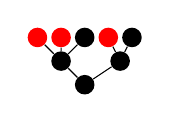
\begin{tikzpicture}[scale=.2]
\node[circle, scale=0.75, fill] (tid0) at (3.75,0){};
\node[circle, scale=0.75, fill] (tid1) at (2.25,1.5){};
\node[circle, scale=0.75, fill, red] (tid3) at (0.75,3){};
\node[circle, scale=0.75, fill, red] (tid4) at (2.25,3){};
\node[circle, scale=0.75, fill] (tid5) at (3.75,3){};
\draw[](tid1) -- (tid3);
\draw[](tid1) -- (tid4);
\draw[](tid1) -- (tid5);
\node[circle, scale=0.75, fill] (tid2) at (6,1.5){};
\node[circle, scale=0.75, fill, red] (tid6) at (5.25,3){};
\node[circle, scale=0.75, fill] (tid7) at (6.75,3){};
\draw[](tid2) -- (tid6);
\draw[](tid2) -- (tid7);
\draw[](tid0) -- (tid1);
\draw[](tid0) -- (tid2);

\end{tikzpicture}
\nodepart{two}
\footnotesize{4.71914}
\nodepart{three}
\footnotesize{$17\:17\:67$}
};
\draw (sn0x8d75fb0W6.south) -- (sn0x8d76e58W-9.north);
\draw (sn0x8d75fb0W6.south) -- (sn0x8d78b18W-1.north);
\draw (sn0x8d75fb0W6.south) -- (sn0x8d78f78W6.north);
\node[draw=black, rectangle split, rectangle split parts=3] (sn0x8d76718W16) at (16, -30) {
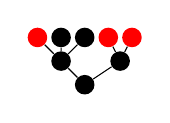
\begin{tikzpicture}[scale=.2]
\node[circle, scale=0.75, fill] (tid0) at (3.75,0){};
\node[circle, scale=0.75, fill] (tid1) at (2.25,1.5){};
\node[circle, scale=0.75, fill, red] (tid3) at (0.75,3){};
\node[circle, scale=0.75, fill] (tid4) at (2.25,3){};
\node[circle, scale=0.75, fill] (tid5) at (3.75,3){};
\draw[](tid1) -- (tid3);
\draw[](tid1) -- (tid4);
\draw[](tid1) -- (tid5);
\node[circle, scale=0.75, fill] (tid2) at (6,1.5){};
\node[circle, scale=0.75, fill, red] (tid6) at (5.25,3){};
\node[circle, scale=0.75, fill, red] (tid7) at (6.75,3){};
\draw[](tid2) -- (tid6);
\draw[](tid2) -- (tid7);
\draw[](tid0) -- (tid1);
\draw[](tid0) -- (tid2);

\end{tikzpicture}
\nodepart{two}
\footnotesize{4.70988}
\nodepart{three}
\footnotesize{$67\:33$}
};
\draw (sn0x8d76718W16.south) -- (sn0x8d76e58W-9.north);
\draw (sn0x8d76718W16.south) -- (sn0x8d78f78W6.north);
\draw (sn0x8d72c50W-4.south) -- (sn0x8d75c30W-25.north);
\draw (sn0x8d72c50W-4.south) -- (sn0x8d75280W-17.north);
\draw (sn0x8d72c50W-4.south) -- (sn0x8d75918W-9.north);
\draw (sn0x8d72c50W-4.south) -- (sn0x8d718a8W-1.north);
\draw (sn0x8d72c50W-4.south) -- (sn0x8d75fb0W6.north);
\draw (sn0x8d72c50W-4.south) -- (sn0x8d76718W16.north);
\end{tikzpicture}

%%% Local Variables:
%%% TeX-master: "thesis/thesis.tex"
%%% End: 

\begin{tikzpicture}[scale=.2, anchor=south west]
\node[draw=black, rectangle split, rectangle split parts=3] (sn0x8d72cb0W-4) at (-4.75, -15) {
\begin{tikzpicture}[scale=.2]
\node[circle, scale=0.75, fill] (tid0) at (3.75,0){};
\node[circle, scale=0.75, fill] (tid1) at (2.25,1.5){};
\node[circle, scale=0.75, fill] (tid3) at (0.75,3){};
\node[circle, scale=0.75, fill, red] (tid8) at (0.75,4.5){};
\draw[](tid3) -- (tid8);
\node[circle, scale=0.75, fill, red] (tid4) at (2.25,3){};
\node[circle, scale=0.75, fill, red] (tid5) at (3.75,3){};
\draw[](tid1) -- (tid3);
\draw[](tid1) -- (tid4);
\draw[](tid1) -- (tid5);
\node[circle, scale=0.75, fill] (tid2) at (6,1.5){};
\node[circle, scale=0.75, fill] (tid6) at (5.25,3){};
\node[circle, scale=0.75, fill] (tid7) at (6.75,3){};
\draw[](tid2) -- (tid6);
\draw[](tid2) -- (tid7);
\draw[](tid0) -- (tid1);
\draw[](tid0) -- (tid2);

\end{tikzpicture}
\nodepart{two}
\footnotesize{5.16135}
\nodepart{three}
\footnotesize{$67\:11\:22$}
};
\node[draw=black, rectangle split, rectangle split parts=3] (sn0x8d75c30W-13) at (-13.5, -30) {
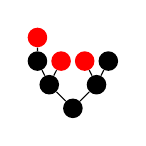
\begin{tikzpicture}[scale=.2]
\node[circle, scale=0.75, fill] (tid0) at (3,0){};
\node[circle, scale=0.75, fill] (tid1) at (1.5,1.5){};
\node[circle, scale=0.75, fill] (tid3) at (0.75,3){};
\node[circle, scale=0.75, fill, red] (tid7) at (0.75,4.5){};
\draw[](tid3) -- (tid7);
\node[circle, scale=0.75, fill, red] (tid4) at (2.25,3){};
\draw[](tid1) -- (tid3);
\draw[](tid1) -- (tid4);
\node[circle, scale=0.75, fill] (tid2) at (4.5,1.5){};
\node[circle, scale=0.75, fill, red] (tid5) at (3.75,3){};
\node[circle, scale=0.75, fill] (tid6) at (5.25,3){};
\draw[](tid2) -- (tid5);
\draw[](tid2) -- (tid6);
\draw[](tid0) -- (tid1);
\draw[](tid0) -- (tid2);

\end{tikzpicture}
\nodepart{two}
\footnotesize{4.88195}
\nodepart{three}
\footnotesize{$33\:33\:33$}
};
\node[draw=black, rectangle split, rectangle split parts=3] (sn0x8d767d0W-18) at (-18.5, -45) {
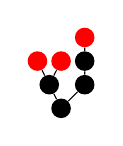
\begin{tikzpicture}[scale=.2]
\node[circle, scale=0.75, fill] (tid0) at (2.25,0){};
\node[circle, scale=0.75, fill] (tid1) at (1.5,1.5){};
\node[circle, scale=0.75, fill, red] (tid3) at (0.75,3){};
\node[circle, scale=0.75, fill, red] (tid4) at (2.25,3){};
\draw[](tid1) -- (tid3);
\draw[](tid1) -- (tid4);
\node[circle, scale=0.75, fill] (tid2) at (3.75,1.5){};
\node[circle, scale=0.75, fill] (tid5) at (3.75,3){};
\node[circle, scale=0.75, fill, red] (tid6) at (3.75,4.5){};
\draw[](tid5) -- (tid6);
\draw[](tid2) -- (tid5);
\draw[](tid0) -- (tid1);
\draw[](tid0) -- (tid2);

\end{tikzpicture}
\nodepart{two}
\footnotesize{4.64352}
\nodepart{three}
\footnotesize{$67\:33$}
};
\node[draw=black, rectangle split, rectangle split parts=3] (sn0x8d77318W-13) at (-13, -60) {
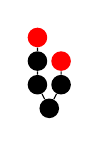
\begin{tikzpicture}[scale=.2]
\node[circle, scale=0.75, fill] (tid0) at (1.5,0){};
\node[circle, scale=0.75, fill] (tid1) at (0.75,1.5){};
\node[circle, scale=0.75, fill] (tid3) at (0.75,3){};
\node[circle, scale=0.75, fill, red] (tid5) at (0.75,4.5){};
\draw[](tid3) -- (tid5);
\draw[](tid1) -- (tid3);
\node[circle, scale=0.75, fill] (tid2) at (2.25,1.5){};
\node[circle, scale=0.75, fill, red] (tid4) at (2.25,3){};
\draw[](tid2) -- (tid4);
\draw[](tid0) -- (tid1);
\draw[](tid0) -- (tid2);

\end{tikzpicture}
\nodepart{two}
\footnotesize{4.4375}
\nodepart{three}
\footnotesize{$50\:50$}
};
\node[draw=black, rectangle split, rectangle split parts=3] (sn0x8d77448W-10) at (-10.75, -75) {
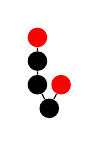
\begin{tikzpicture}[scale=.2]
\node[circle, scale=0.75, fill] (tid0) at (1.5,0){};
\node[circle, scale=0.75, fill] (tid1) at (0.75,1.5){};
\node[circle, scale=0.75, fill] (tid3) at (0.75,3){};
\node[circle, scale=0.75, fill, red] (tid4) at (0.75,4.5){};
\draw[](tid3) -- (tid4);
\draw[](tid1) -- (tid3);
\node[circle, scale=0.75, fill, red] (tid2) at (2.25,1.5){};
\draw[](tid0) -- (tid1);
\draw[](tid0) -- (tid2);

\end{tikzpicture}
\nodepart{two}
\footnotesize{4.125}
\nodepart{three}
\footnotesize{$50\:50$}
};
\node[draw=black, rectangle split, rectangle split parts=3] (sn0x8d77658W-6) at (-6.75, -90) {
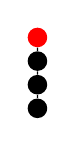
\begin{tikzpicture}[scale=.2]
\node[circle, scale=0.75, fill] (tid0) at (0.75,0){};
\node[circle, scale=0.75, fill] (tid1) at (0.75,1.5){};
\node[circle, scale=0.75, fill] (tid2) at (0.75,3){};
\node[circle, scale=0.75, fill, red] (tid3) at (0.75,4.5){};
\draw[](tid2) -- (tid3);
\draw[](tid1) -- (tid2);
\draw[](tid0) -- (tid1);

\end{tikzpicture}
\nodepart{two}
\footnotesize{4}
\nodepart{three}
\footnotesize{$1$}
};
\node[draw=black, rectangle split, rectangle split parts=3] (sn0x8d77980W-4) at (-4.25, -105) {
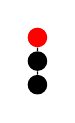
\begin{tikzpicture}[scale=.2]
\node[circle, scale=0.75, fill] (tid0) at (0.75,0){};
\node[circle, scale=0.75, fill] (tid1) at (0.75,1.5){};
\node[circle, scale=0.75, fill, red] (tid2) at (0.75,3){};
\draw[](tid1) -- (tid2);
\draw[](tid0) -- (tid1);

\end{tikzpicture}
\nodepart{two}
\footnotesize{3}
\nodepart{three}
\footnotesize{$1$}
};
\node[draw=black, rectangle split, rectangle split parts=3] (sn0x8d77af8W-1) at (-1.75, -120) {

\begin{tikzpicture}[scale=.2]
\node[circle, scale=0.75, fill] (tid0) at (0.75,0){};
\node[circle, scale=0.75, fill, red] (tid1) at (0.75,1.5){};
\draw[](tid0) -- (tid1);

\end{tikzpicture}
\nodepart{two}
\footnotesize{2}
\nodepart{three}
\footnotesize{$1$}
};
\draw (sn0x8d77980W-4.south) -- (sn0x8d77af8W-1.north);
\draw (sn0x8d77658W-6.south) -- (sn0x8d77980W-4.north);
\node[draw=black, rectangle split, rectangle split parts=3] (sn0x8d77810W-3) at (-3.25, -90) {
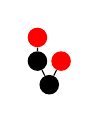
\begin{tikzpicture}[scale=.2]
\node[circle, scale=0.75, fill] (tid0) at (1.5,0){};
\node[circle, scale=0.75, fill] (tid1) at (0.75,1.5){};
\node[circle, scale=0.75, fill, red] (tid3) at (0.75,3){};
\draw[](tid1) -- (tid3);
\node[circle, scale=0.75, fill, red] (tid2) at (2.25,1.5){};
\draw[](tid0) -- (tid1);
\draw[](tid0) -- (tid2);

\end{tikzpicture}
\nodepart{two}
\footnotesize{3.25}
\nodepart{three}
\footnotesize{$50\:50$}
};
\node[draw=black, rectangle split, rectangle split parts=3] (sn0x8d77cb8W0) at (-0.75, -105) {

\begin{tikzpicture}[scale=.2]
\node[circle, scale=0.75, fill] (tid0) at (1.5,0){};
\node[circle, scale=0.75, fill, red] (tid1) at (0.75,1.5){};
\node[circle, scale=0.75, fill, red] (tid2) at (2.25,1.5){};
\draw[](tid0) -- (tid1);
\draw[](tid0) -- (tid2);

\end{tikzpicture}
\nodepart{two}
\footnotesize{2.5}
\nodepart{three}
\footnotesize{$1$}
};
\draw (sn0x8d77cb8W0.south) -- (sn0x8d77af8W-1.north);
\draw (sn0x8d77810W-3.south) -- (sn0x8d77980W-4.north);
\draw (sn0x8d77810W-3.south) -- (sn0x8d77cb8W0.north);
\draw (sn0x8d77448W-10.south) -- (sn0x8d77658W-6.north);
\draw (sn0x8d77448W-10.south) -- (sn0x8d77810W-3.north);
\node[draw=black, rectangle split, rectangle split parts=3] (sn0x8d775f0W-5) at (-5.75, -75) {
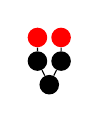
\begin{tikzpicture}[scale=.2]
\node[circle, scale=0.75, fill] (tid0) at (1.5,0){};
\node[circle, scale=0.75, fill] (tid1) at (0.75,1.5){};
\node[circle, scale=0.75, fill, red] (tid3) at (0.75,3){};
\draw[](tid1) -- (tid3);
\node[circle, scale=0.75, fill] (tid2) at (2.25,1.5){};
\node[circle, scale=0.75, fill, red] (tid4) at (2.25,3){};
\draw[](tid2) -- (tid4);
\draw[](tid0) -- (tid1);
\draw[](tid0) -- (tid2);

\end{tikzpicture}
\nodepart{two}
\footnotesize{3.75}
\nodepart{three}
\footnotesize{$1$}
};
\draw (sn0x8d775f0W-5.south) -- (sn0x8d77810W-3.north);
\draw (sn0x8d77318W-13.south) -- (sn0x8d77448W-10.north);
\draw (sn0x8d77318W-13.south) -- (sn0x8d775f0W-5.north);
\node[draw=black, rectangle split, rectangle split parts=3] (sn0x8d773b0W-8) at (-8, -60) {
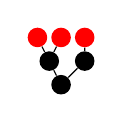
\begin{tikzpicture}[scale=.2]
\node[circle, scale=0.75, fill] (tid0) at (2.25,0){};
\node[circle, scale=0.75, fill] (tid1) at (1.5,1.5){};
\node[circle, scale=0.75, fill, red] (tid3) at (0.75,3){};
\node[circle, scale=0.75, fill, red] (tid4) at (2.25,3){};
\draw[](tid1) -- (tid3);
\draw[](tid1) -- (tid4);
\node[circle, scale=0.75, fill] (tid2) at (3.75,1.5){};
\node[circle, scale=0.75, fill, red] (tid5) at (3.75,3){};
\draw[](tid2) -- (tid5);
\draw[](tid0) -- (tid1);
\draw[](tid0) -- (tid2);

\end{tikzpicture}
\nodepart{two}
\footnotesize{4.05556}
\nodepart{three}
\footnotesize{$67\:33$}
};
\node[draw=black, rectangle split, rectangle split parts=3] (sn0x8d78058W0) at (-0.75, -75) {
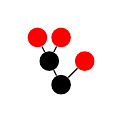
\begin{tikzpicture}[scale=.2]
\node[circle, scale=0.75, fill] (tid0) at (2.25,0){};
\node[circle, scale=0.75, fill] (tid1) at (1.5,1.5){};
\node[circle, scale=0.75, fill, red] (tid3) at (0.75,3){};
\node[circle, scale=0.75, fill, red] (tid4) at (2.25,3){};
\draw[](tid1) -- (tid3);
\draw[](tid1) -- (tid4);
\node[circle, scale=0.75, fill, red] (tid2) at (3.75,1.5){};
\draw[](tid0) -- (tid1);
\draw[](tid0) -- (tid2);

\end{tikzpicture}
\nodepart{two}
\footnotesize{3.66667}
\nodepart{three}
\footnotesize{$67\:33$}
};
\node[draw=black, rectangle split, rectangle split parts=3] (sn0x8d781a8W1) at (1.75, -90) {
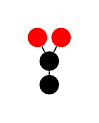
\begin{tikzpicture}[scale=.2]
\node[circle, scale=0.75, fill] (tid0) at (1.5,0){};
\node[circle, scale=0.75, fill] (tid1) at (1.5,1.5){};
\node[circle, scale=0.75, fill, red] (tid2) at (0.75,3){};
\node[circle, scale=0.75, fill, red] (tid3) at (2.25,3){};
\draw[](tid1) -- (tid2);
\draw[](tid1) -- (tid3);
\draw[](tid0) -- (tid1);

\end{tikzpicture}
\nodepart{two}
\footnotesize{3.5}
\nodepart{three}
\footnotesize{$1$}
};
\draw (sn0x8d781a8W1.south) -- (sn0x8d77980W-4.north);
\draw (sn0x8d78058W0.south) -- (sn0x8d781a8W1.north);
\draw (sn0x8d78058W0.south) -- (sn0x8d77810W-3.north);
\draw (sn0x8d773b0W-8.south) -- (sn0x8d775f0W-5.north);
\draw (sn0x8d773b0W-8.south) -- (sn0x8d78058W0.north);
\draw (sn0x8d767d0W-18.south) -- (sn0x8d77318W-13.north);
\draw (sn0x8d767d0W-18.south) -- (sn0x8d773b0W-8.north);
\node[draw=black, rectangle split, rectangle split parts=3] (sn0x8d76d60W-12) at (-12, -45) {
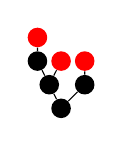
\begin{tikzpicture}[scale=.2]
\node[circle, scale=0.75, fill] (tid0) at (2.25,0){};
\node[circle, scale=0.75, fill] (tid1) at (1.5,1.5){};
\node[circle, scale=0.75, fill] (tid3) at (0.75,3){};
\node[circle, scale=0.75, fill, red] (tid6) at (0.75,4.5){};
\draw[](tid3) -- (tid6);
\node[circle, scale=0.75, fill, red] (tid4) at (2.25,3){};
\draw[](tid1) -- (tid3);
\draw[](tid1) -- (tid4);
\node[circle, scale=0.75, fill] (tid2) at (3.75,1.5){};
\node[circle, scale=0.75, fill, red] (tid5) at (3.75,3){};
\draw[](tid2) -- (tid5);
\draw[](tid0) -- (tid1);
\draw[](tid0) -- (tid2);

\end{tikzpicture}
\nodepart{two}
\footnotesize{4.61343}
\nodepart{three}
\footnotesize{$33\:33\:33$}
};
\node[draw=black, rectangle split, rectangle split parts=3] (sn0x8d78990W-1) at (-1.5, -60) {
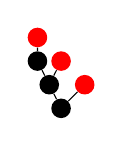
\begin{tikzpicture}[scale=.2]
\node[circle, scale=0.75, fill] (tid0) at (2.25,0){};
\node[circle, scale=0.75, fill] (tid1) at (1.5,1.5){};
\node[circle, scale=0.75, fill] (tid3) at (0.75,3){};
\node[circle, scale=0.75, fill, red] (tid5) at (0.75,4.5){};
\draw[](tid3) -- (tid5);
\node[circle, scale=0.75, fill, red] (tid4) at (2.25,3){};
\draw[](tid1) -- (tid3);
\draw[](tid1) -- (tid4);
\node[circle, scale=0.75, fill, red] (tid2) at (3.75,1.5){};
\draw[](tid0) -- (tid1);
\draw[](tid0) -- (tid2);

\end{tikzpicture}
\nodepart{two}
\footnotesize{4.34722}
\nodepart{three}
\footnotesize{$33\:33\:33$}
};
\node[draw=black, rectangle split, rectangle split parts=3] (sn0x8d78430W5) at (5.75, -75) {
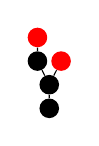
\begin{tikzpicture}[scale=.2]
\node[circle, scale=0.75, fill] (tid0) at (1.5,0){};
\node[circle, scale=0.75, fill] (tid1) at (1.5,1.5){};
\node[circle, scale=0.75, fill] (tid2) at (0.75,3){};
\node[circle, scale=0.75, fill, red] (tid4) at (0.75,4.5){};
\draw[](tid2) -- (tid4);
\node[circle, scale=0.75, fill, red] (tid3) at (2.25,3){};
\draw[](tid1) -- (tid2);
\draw[](tid1) -- (tid3);
\draw[](tid0) -- (tid1);

\end{tikzpicture}
\nodepart{two}
\footnotesize{4.25}
\nodepart{three}
\footnotesize{$50\:50$}
};
\draw (sn0x8d78430W5.south) -- (sn0x8d77658W-6.north);
\draw (sn0x8d78430W5.south) -- (sn0x8d781a8W1.north);
\draw (sn0x8d78990W-1.south) -- (sn0x8d78430W5.north);
\draw (sn0x8d78990W-1.south) -- (sn0x8d77448W-10.north);
\draw (sn0x8d78990W-1.south) -- (sn0x8d78058W0.north);
\draw (sn0x8d76d60W-12.south) -- (sn0x8d77318W-13.north);
\draw (sn0x8d76d60W-12.south) -- (sn0x8d78990W-1.north);
\draw (sn0x8d76d60W-12.south) -- (sn0x8d773b0W-8.north);
\node[draw=black, rectangle split, rectangle split parts=3] (sn0x8d76e58W-5) at (-5.5, -45) {
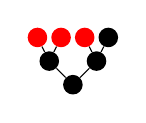
\begin{tikzpicture}[scale=.2]
\node[circle, scale=0.75, fill] (tid0) at (3,0){};
\node[circle, scale=0.75, fill] (tid1) at (1.5,1.5){};
\node[circle, scale=0.75, fill, red] (tid3) at (0.75,3){};
\node[circle, scale=0.75, fill, red] (tid4) at (2.25,3){};
\draw[](tid1) -- (tid3);
\draw[](tid1) -- (tid4);
\node[circle, scale=0.75, fill] (tid2) at (4.5,1.5){};
\node[circle, scale=0.75, fill, red] (tid5) at (3.75,3){};
\node[circle, scale=0.75, fill] (tid6) at (5.25,3){};
\draw[](tid2) -- (tid5);
\draw[](tid2) -- (tid6);
\draw[](tid0) -- (tid1);
\draw[](tid0) -- (tid2);

\end{tikzpicture}
\nodepart{two}
\footnotesize{4.38889}
\nodepart{three}
\footnotesize{$1$}
};
\draw (sn0x8d76e58W-5.south) -- (sn0x8d773b0W-8.north);
\draw (sn0x8d75c30W-13.south) -- (sn0x8d767d0W-18.north);
\draw (sn0x8d75c30W-13.south) -- (sn0x8d76d60W-12.north);
\draw (sn0x8d75c30W-13.south) -- (sn0x8d76e58W-5.north);
\node[draw=black, rectangle split, rectangle split parts=3] (sn0x8d795c0W-5) at (-5.5, -30) {
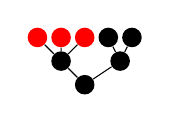
\begin{tikzpicture}[scale=.2]
\node[circle, scale=0.75, fill] (tid0) at (3.75,0){};
\node[circle, scale=0.75, fill] (tid1) at (2.25,1.5){};
\node[circle, scale=0.75, fill, red] (tid3) at (0.75,3){};
\node[circle, scale=0.75, fill, red] (tid4) at (2.25,3){};
\node[circle, scale=0.75, fill, red] (tid5) at (3.75,3){};
\draw[](tid1) -- (tid3);
\draw[](tid1) -- (tid4);
\draw[](tid1) -- (tid5);
\node[circle, scale=0.75, fill] (tid2) at (6,1.5){};
\node[circle, scale=0.75, fill] (tid6) at (5.25,3){};
\node[circle, scale=0.75, fill] (tid7) at (6.75,3){};
\draw[](tid2) -- (tid6);
\draw[](tid2) -- (tid7);
\draw[](tid0) -- (tid1);
\draw[](tid0) -- (tid2);

\end{tikzpicture}
\nodepart{two}
\footnotesize{4.72222}
\nodepart{three}
\footnotesize{$1$}
};
\draw (sn0x8d795c0W-5.south) -- (sn0x8d76e58W-5.north);
\node[draw=black, rectangle split, rectangle split parts=3] (sn0x8d75fb0W4) at (4, -30) {
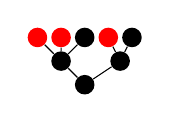
\begin{tikzpicture}[scale=.2]
\node[circle, scale=0.75, fill] (tid0) at (3.75,0){};
\node[circle, scale=0.75, fill] (tid1) at (2.25,1.5){};
\node[circle, scale=0.75, fill, red] (tid3) at (0.75,3){};
\node[circle, scale=0.75, fill, red] (tid4) at (2.25,3){};
\node[circle, scale=0.75, fill] (tid5) at (3.75,3){};
\draw[](tid1) -- (tid3);
\draw[](tid1) -- (tid4);
\draw[](tid1) -- (tid5);
\node[circle, scale=0.75, fill] (tid2) at (6,1.5){};
\node[circle, scale=0.75, fill, red] (tid6) at (5.25,3){};
\node[circle, scale=0.75, fill] (tid7) at (6.75,3){};
\draw[](tid2) -- (tid6);
\draw[](tid2) -- (tid7);
\draw[](tid0) -- (tid1);
\draw[](tid0) -- (tid2);

\end{tikzpicture}
\nodepart{two}
\footnotesize{4.71914}
\nodepart{three}
\footnotesize{$67\:17\:17$}
};
\node[draw=black, rectangle split, rectangle split parts=3] (sn0x8d78b18W2) at (2.5, -45) {
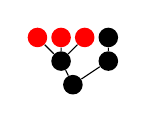
\begin{tikzpicture}[scale=.2]
\node[circle, scale=0.75, fill] (tid0) at (3,0){};
\node[circle, scale=0.75, fill] (tid1) at (2.25,1.5){};
\node[circle, scale=0.75, fill, red] (tid3) at (0.75,3){};
\node[circle, scale=0.75, fill, red] (tid4) at (2.25,3){};
\node[circle, scale=0.75, fill, red] (tid5) at (3.75,3){};
\draw[](tid1) -- (tid3);
\draw[](tid1) -- (tid4);
\draw[](tid1) -- (tid5);
\node[circle, scale=0.75, fill] (tid2) at (5.25,1.5){};
\node[circle, scale=0.75, fill] (tid6) at (5.25,3){};
\draw[](tid2) -- (tid6);
\draw[](tid0) -- (tid1);
\draw[](tid0) -- (tid2);

\end{tikzpicture}
\nodepart{two}
\footnotesize{4.38889}
\nodepart{three}
\footnotesize{$1$}
};
\draw (sn0x8d78b18W2.south) -- (sn0x8d773b0W-8.north);
\node[draw=black, rectangle split, rectangle split parts=3] (sn0x8d78f78W10) at (10.5, -45) {
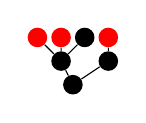
\begin{tikzpicture}[scale=.2]
\node[circle, scale=0.75, fill] (tid0) at (3,0){};
\node[circle, scale=0.75, fill] (tid1) at (2.25,1.5){};
\node[circle, scale=0.75, fill, red] (tid3) at (0.75,3){};
\node[circle, scale=0.75, fill, red] (tid4) at (2.25,3){};
\node[circle, scale=0.75, fill] (tid5) at (3.75,3){};
\draw[](tid1) -- (tid3);
\draw[](tid1) -- (tid4);
\draw[](tid1) -- (tid5);
\node[circle, scale=0.75, fill] (tid2) at (5.25,1.5){};
\node[circle, scale=0.75, fill, red] (tid6) at (5.25,3){};
\draw[](tid2) -- (tid6);
\draw[](tid0) -- (tid1);
\draw[](tid0) -- (tid2);

\end{tikzpicture}
\nodepart{two}
\footnotesize{4.37037}
\nodepart{three}
\footnotesize{$67\:33$}
};
\node[draw=black, rectangle split, rectangle split parts=3] (sn0x8d78a68W5) at (5, -60) {
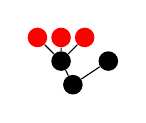
\begin{tikzpicture}[scale=.2]
\node[circle, scale=0.75, fill] (tid0) at (3,0){};
\node[circle, scale=0.75, fill] (tid1) at (2.25,1.5){};
\node[circle, scale=0.75, fill, red] (tid3) at (0.75,3){};
\node[circle, scale=0.75, fill, red] (tid4) at (2.25,3){};
\node[circle, scale=0.75, fill, red] (tid5) at (3.75,3){};
\draw[](tid1) -- (tid3);
\draw[](tid1) -- (tid4);
\draw[](tid1) -- (tid5);
\node[circle, scale=0.75, fill] (tid2) at (5.25,1.5){};
\draw[](tid0) -- (tid1);
\draw[](tid0) -- (tid2);

\end{tikzpicture}
\nodepart{two}
\footnotesize{4}
\nodepart{three}
\footnotesize{$1$}
};
\draw (sn0x8d78a68W5.south) -- (sn0x8d78058W0.north);
\draw (sn0x8d78f78W10.south) -- (sn0x8d773b0W-8.north);
\draw (sn0x8d78f78W10.south) -- (sn0x8d78a68W5.north);
\draw (sn0x8d75fb0W4.south) -- (sn0x8d76e58W-5.north);
\draw (sn0x8d75fb0W4.south) -- (sn0x8d78b18W2.north);
\draw (sn0x8d75fb0W4.south) -- (sn0x8d78f78W10.north);
\draw (sn0x8d72cb0W-4.south) -- (sn0x8d75c30W-13.north);
\draw (sn0x8d72cb0W-4.south) -- (sn0x8d795c0W-5.north);
\draw (sn0x8d72cb0W-4.south) -- (sn0x8d75fb0W4.north);
\end{tikzpicture}

%%% Local Variables:
%%% TeX-master: "thesis/thesis.tex"
%%% End: 

\begin{tikzpicture}[scale=.2, anchor=south west]
\node[draw=black, rectangle split, rectangle split parts=3] (sn0x8d72d10W-4) at (-4.75, -15) {
\begin{tikzpicture}[scale=.2]
\node[circle, scale=0.75, fill] (tid0) at (3.75,0){};
\node[circle, scale=0.75, fill] (tid1) at (2.25,1.5){};
\node[circle, scale=0.75, fill] (tid3) at (0.75,3){};
\node[circle, scale=0.75, fill, red] (tid8) at (0.75,4.5){};
\draw[](tid3) -- (tid8);
\node[circle, scale=0.75, fill] (tid4) at (2.25,3){};
\node[circle, scale=0.75, fill] (tid5) at (3.75,3){};
\draw[](tid1) -- (tid3);
\draw[](tid1) -- (tid4);
\draw[](tid1) -- (tid5);
\node[circle, scale=0.75, fill] (tid2) at (6,1.5){};
\node[circle, scale=0.75, fill, red] (tid6) at (5.25,3){};
\node[circle, scale=0.75, fill, red] (tid7) at (6.75,3){};
\draw[](tid2) -- (tid6);
\draw[](tid2) -- (tid7);
\draw[](tid0) -- (tid1);
\draw[](tid0) -- (tid2);

\end{tikzpicture}
\nodepart{two}
\footnotesize{5.13632}
\nodepart{three}
\footnotesize{$67\:33$}
};
\node[draw=black, rectangle split, rectangle split parts=3] (sn0x8d718a8W-8) at (-8.75, -30) {
\begin{tikzpicture}[scale=.2]
\node[circle, scale=0.75, fill] (tid0) at (3,0){};
\node[circle, scale=0.75, fill] (tid1) at (2.25,1.5){};
\node[circle, scale=0.75, fill] (tid3) at (0.75,3){};
\node[circle, scale=0.75, fill, red] (tid7) at (0.75,4.5){};
\draw[](tid3) -- (tid7);
\node[circle, scale=0.75, fill, red] (tid4) at (2.25,3){};
\node[circle, scale=0.75, fill] (tid5) at (3.75,3){};
\draw[](tid1) -- (tid3);
\draw[](tid1) -- (tid4);
\draw[](tid1) -- (tid5);
\node[circle, scale=0.75, fill] (tid2) at (5.25,1.5){};
\node[circle, scale=0.75, fill, red] (tid6) at (5.25,3){};
\draw[](tid2) -- (tid6);
\draw[](tid0) -- (tid1);
\draw[](tid0) -- (tid2);

\end{tikzpicture}
\nodepart{two}
\footnotesize{4.84954}
\nodepart{three}
\footnotesize{$33\:33\:33$}
};
\node[draw=black, rectangle split, rectangle split parts=3] (sn0x8d76d60W-15) at (-15.25, -45) {
\begin{tikzpicture}[scale=.2]
\node[circle, scale=0.75, fill] (tid0) at (2.25,0){};
\node[circle, scale=0.75, fill] (tid1) at (1.5,1.5){};
\node[circle, scale=0.75, fill] (tid3) at (0.75,3){};
\node[circle, scale=0.75, fill, red] (tid6) at (0.75,4.5){};
\draw[](tid3) -- (tid6);
\node[circle, scale=0.75, fill, red] (tid4) at (2.25,3){};
\draw[](tid1) -- (tid3);
\draw[](tid1) -- (tid4);
\node[circle, scale=0.75, fill] (tid2) at (3.75,1.5){};
\node[circle, scale=0.75, fill, red] (tid5) at (3.75,3){};
\draw[](tid2) -- (tid5);
\draw[](tid0) -- (tid1);
\draw[](tid0) -- (tid2);

\end{tikzpicture}
\nodepart{two}
\footnotesize{4.61343}
\nodepart{three}
\footnotesize{$33\:33\:33$}
};
\node[draw=black, rectangle split, rectangle split parts=3] (sn0x8d77318W-13) at (-13, -60) {
\begin{tikzpicture}[scale=.2]
\node[circle, scale=0.75, fill] (tid0) at (1.5,0){};
\node[circle, scale=0.75, fill] (tid1) at (0.75,1.5){};
\node[circle, scale=0.75, fill] (tid3) at (0.75,3){};
\node[circle, scale=0.75, fill, red] (tid5) at (0.75,4.5){};
\draw[](tid3) -- (tid5);
\draw[](tid1) -- (tid3);
\node[circle, scale=0.75, fill] (tid2) at (2.25,1.5){};
\node[circle, scale=0.75, fill, red] (tid4) at (2.25,3){};
\draw[](tid2) -- (tid4);
\draw[](tid0) -- (tid1);
\draw[](tid0) -- (tid2);

\end{tikzpicture}
\nodepart{two}
\footnotesize{4.4375}
\nodepart{three}
\footnotesize{$50\:50$}
};
\node[draw=black, rectangle split, rectangle split parts=3] (sn0x8d77448W-10) at (-10.75, -75) {
\begin{tikzpicture}[scale=.2]
\node[circle, scale=0.75, fill] (tid0) at (1.5,0){};
\node[circle, scale=0.75, fill] (tid1) at (0.75,1.5){};
\node[circle, scale=0.75, fill] (tid3) at (0.75,3){};
\node[circle, scale=0.75, fill, red] (tid4) at (0.75,4.5){};
\draw[](tid3) -- (tid4);
\draw[](tid1) -- (tid3);
\node[circle, scale=0.75, fill, red] (tid2) at (2.25,1.5){};
\draw[](tid0) -- (tid1);
\draw[](tid0) -- (tid2);

\end{tikzpicture}
\nodepart{two}
\footnotesize{4.125}
\nodepart{three}
\footnotesize{$50\:50$}
};
\node[draw=black, rectangle split, rectangle split parts=3] (sn0x8d77658W-6) at (-6.75, -90) {
\begin{tikzpicture}[scale=.2]
\node[circle, scale=0.75, fill] (tid0) at (0.75,0){};
\node[circle, scale=0.75, fill] (tid1) at (0.75,1.5){};
\node[circle, scale=0.75, fill] (tid2) at (0.75,3){};
\node[circle, scale=0.75, fill, red] (tid3) at (0.75,4.5){};
\draw[](tid2) -- (tid3);
\draw[](tid1) -- (tid2);
\draw[](tid0) -- (tid1);

\end{tikzpicture}
\nodepart{two}
\footnotesize{4}
\nodepart{three}
\footnotesize{$1$}
};
\node[draw=black, rectangle split, rectangle split parts=3] (sn0x8d77980W-4) at (-4.25, -105) {
\begin{tikzpicture}[scale=.2]
\node[circle, scale=0.75, fill] (tid0) at (0.75,0){};
\node[circle, scale=0.75, fill] (tid1) at (0.75,1.5){};
\node[circle, scale=0.75, fill, red] (tid2) at (0.75,3){};
\draw[](tid1) -- (tid2);
\draw[](tid0) -- (tid1);

\end{tikzpicture}
\nodepart{two}
\footnotesize{3}
\nodepart{three}
\footnotesize{$1$}
};
\node[draw=black, rectangle split, rectangle split parts=3] (sn0x8d77af8W-1) at (-1.75, -120) {
\begin{tikzpicture}[scale=.2]
\node[circle, scale=0.75, fill] (tid0) at (0.75,0){};
\node[circle, scale=0.75, fill, red] (tid1) at (0.75,1.5){};
\draw[](tid0) -- (tid1);

\end{tikzpicture}
\nodepart{two}
\footnotesize{2}
\nodepart{three}
\footnotesize{$1$}
};
\draw (sn0x8d77980W-4.south) -- (sn0x8d77af8W-1.north);
\draw (sn0x8d77658W-6.south) -- (sn0x8d77980W-4.north);
\node[draw=black, rectangle split, rectangle split parts=3] (sn0x8d77810W-3) at (-3.25, -90) {
\begin{tikzpicture}[scale=.2]
\node[circle, scale=0.75, fill] (tid0) at (1.5,0){};
\node[circle, scale=0.75, fill] (tid1) at (0.75,1.5){};
\node[circle, scale=0.75, fill, red] (tid3) at (0.75,3){};
\draw[](tid1) -- (tid3);
\node[circle, scale=0.75, fill, red] (tid2) at (2.25,1.5){};
\draw[](tid0) -- (tid1);
\draw[](tid0) -- (tid2);

\end{tikzpicture}
\nodepart{two}
\footnotesize{3.25}
\nodepart{three}
\footnotesize{$50\:50$}
};
\node[draw=black, rectangle split, rectangle split parts=3] (sn0x8d77cb8W0) at (-0.75, -105) {
\begin{tikzpicture}[scale=.2]
\node[circle, scale=0.75, fill] (tid0) at (1.5,0){};
\node[circle, scale=0.75, fill, red] (tid1) at (0.75,1.5){};
\node[circle, scale=0.75, fill, red] (tid2) at (2.25,1.5){};
\draw[](tid0) -- (tid1);
\draw[](tid0) -- (tid2);

\end{tikzpicture}
\nodepart{two}
\footnotesize{2.5}
\nodepart{three}
\footnotesize{$1$}
};
\draw (sn0x8d77cb8W0.south) -- (sn0x8d77af8W-1.north);
\draw (sn0x8d77810W-3.south) -- (sn0x8d77980W-4.north);
\draw (sn0x8d77810W-3.south) -- (sn0x8d77cb8W0.north);
\draw (sn0x8d77448W-10.south) -- (sn0x8d77658W-6.north);
\draw (sn0x8d77448W-10.south) -- (sn0x8d77810W-3.north);
\node[draw=black, rectangle split, rectangle split parts=3] (sn0x8d775f0W-5) at (-5.75, -75) {
\begin{tikzpicture}[scale=.2]
\node[circle, scale=0.75, fill] (tid0) at (1.5,0){};
\node[circle, scale=0.75, fill] (tid1) at (0.75,1.5){};
\node[circle, scale=0.75, fill, red] (tid3) at (0.75,3){};
\draw[](tid1) -- (tid3);
\node[circle, scale=0.75, fill] (tid2) at (2.25,1.5){};
\node[circle, scale=0.75, fill, red] (tid4) at (2.25,3){};
\draw[](tid2) -- (tid4);
\draw[](tid0) -- (tid1);
\draw[](tid0) -- (tid2);

\end{tikzpicture}
\nodepart{two}
\footnotesize{3.75}
\nodepart{three}
\footnotesize{$1$}
};
\draw (sn0x8d775f0W-5.south) -- (sn0x8d77810W-3.north);
\draw (sn0x8d77318W-13.south) -- (sn0x8d77448W-10.north);
\draw (sn0x8d77318W-13.south) -- (sn0x8d775f0W-5.north);
\node[draw=black, rectangle split, rectangle split parts=3] (sn0x8d78990W-8) at (-8, -60) {
\begin{tikzpicture}[scale=.2]
\node[circle, scale=0.75, fill] (tid0) at (2.25,0){};
\node[circle, scale=0.75, fill] (tid1) at (1.5,1.5){};
\node[circle, scale=0.75, fill] (tid3) at (0.75,3){};
\node[circle, scale=0.75, fill, red] (tid5) at (0.75,4.5){};
\draw[](tid3) -- (tid5);
\node[circle, scale=0.75, fill, red] (tid4) at (2.25,3){};
\draw[](tid1) -- (tid3);
\draw[](tid1) -- (tid4);
\node[circle, scale=0.75, fill, red] (tid2) at (3.75,1.5){};
\draw[](tid0) -- (tid1);
\draw[](tid0) -- (tid2);

\end{tikzpicture}
\nodepart{two}
\footnotesize{4.34722}
\nodepart{three}
\footnotesize{$33\:33\:33$}
};
\node[draw=black, rectangle split, rectangle split parts=3] (sn0x8d78430W0) at (-0.75, -75) {
\begin{tikzpicture}[scale=.2]
\node[circle, scale=0.75, fill] (tid0) at (1.5,0){};
\node[circle, scale=0.75, fill] (tid1) at (1.5,1.5){};
\node[circle, scale=0.75, fill] (tid2) at (0.75,3){};
\node[circle, scale=0.75, fill, red] (tid4) at (0.75,4.5){};
\draw[](tid2) -- (tid4);
\node[circle, scale=0.75, fill, red] (tid3) at (2.25,3){};
\draw[](tid1) -- (tid2);
\draw[](tid1) -- (tid3);
\draw[](tid0) -- (tid1);

\end{tikzpicture}
\nodepart{two}
\footnotesize{4.25}
\nodepart{three}
\footnotesize{$50\:50$}
};
\node[draw=black, rectangle split, rectangle split parts=3] (sn0x8d781a8W1) at (1.75, -90) {
\begin{tikzpicture}[scale=.2]
\node[circle, scale=0.75, fill] (tid0) at (1.5,0){};
\node[circle, scale=0.75, fill] (tid1) at (1.5,1.5){};
\node[circle, scale=0.75, fill, red] (tid2) at (0.75,3){};
\node[circle, scale=0.75, fill, red] (tid3) at (2.25,3){};
\draw[](tid1) -- (tid2);
\draw[](tid1) -- (tid3);
\draw[](tid0) -- (tid1);

\end{tikzpicture}
\nodepart{two}
\footnotesize{3.5}
\nodepart{three}
\footnotesize{$1$}
};
\draw (sn0x8d781a8W1.south) -- (sn0x8d77980W-4.north);
\draw (sn0x8d78430W0.south) -- (sn0x8d77658W-6.north);
\draw (sn0x8d78430W0.south) -- (sn0x8d781a8W1.north);
\node[draw=black, rectangle split, rectangle split parts=3] (sn0x8d78058W4) at (4.25, -75) {
\begin{tikzpicture}[scale=.2]
\node[circle, scale=0.75, fill] (tid0) at (2.25,0){};
\node[circle, scale=0.75, fill] (tid1) at (1.5,1.5){};
\node[circle, scale=0.75, fill, red] (tid3) at (0.75,3){};
\node[circle, scale=0.75, fill, red] (tid4) at (2.25,3){};
\draw[](tid1) -- (tid3);
\draw[](tid1) -- (tid4);
\node[circle, scale=0.75, fill, red] (tid2) at (3.75,1.5){};
\draw[](tid0) -- (tid1);
\draw[](tid0) -- (tid2);

\end{tikzpicture}
\nodepart{two}
\footnotesize{3.66667}
\nodepart{three}
\footnotesize{$33\:67$}
};
\draw (sn0x8d78058W4.south) -- (sn0x8d781a8W1.north);
\draw (sn0x8d78058W4.south) -- (sn0x8d77810W-3.north);
\draw (sn0x8d78990W-8.south) -- (sn0x8d78430W0.north);
\draw (sn0x8d78990W-8.south) -- (sn0x8d77448W-10.north);
\draw (sn0x8d78990W-8.south) -- (sn0x8d78058W4.north);
\node[draw=black, rectangle split, rectangle split parts=3] (sn0x8d773b0W-1) at (-1.5, -60) {
\begin{tikzpicture}[scale=.2]
\node[circle, scale=0.75, fill] (tid0) at (2.25,0){};
\node[circle, scale=0.75, fill] (tid1) at (1.5,1.5){};
\node[circle, scale=0.75, fill, red] (tid3) at (0.75,3){};
\node[circle, scale=0.75, fill, red] (tid4) at (2.25,3){};
\draw[](tid1) -- (tid3);
\draw[](tid1) -- (tid4);
\node[circle, scale=0.75, fill] (tid2) at (3.75,1.5){};
\node[circle, scale=0.75, fill, red] (tid5) at (3.75,3){};
\draw[](tid2) -- (tid5);
\draw[](tid0) -- (tid1);
\draw[](tid0) -- (tid2);

\end{tikzpicture}
\nodepart{two}
\footnotesize{4.05556}
\nodepart{three}
\footnotesize{$33\:67$}
};
\draw (sn0x8d773b0W-1.south) -- (sn0x8d775f0W-5.north);
\draw (sn0x8d773b0W-1.south) -- (sn0x8d78058W4.north);
\draw (sn0x8d76d60W-15.south) -- (sn0x8d77318W-13.north);
\draw (sn0x8d76d60W-15.south) -- (sn0x8d78990W-8.north);
\draw (sn0x8d76d60W-15.south) -- (sn0x8d773b0W-1.north);
\node[draw=black, rectangle split, rectangle split parts=3] (sn0x8d791d0W-8) at (-8.75, -45) {
\begin{tikzpicture}[scale=.2]
\node[circle, scale=0.75, fill] (tid0) at (3,0){};
\node[circle, scale=0.75, fill] (tid1) at (2.25,1.5){};
\node[circle, scale=0.75, fill] (tid3) at (0.75,3){};
\node[circle, scale=0.75, fill, red] (tid6) at (0.75,4.5){};
\draw[](tid3) -- (tid6);
\node[circle, scale=0.75, fill, red] (tid4) at (2.25,3){};
\node[circle, scale=0.75, fill, red] (tid5) at (3.75,3){};
\draw[](tid1) -- (tid3);
\draw[](tid1) -- (tid4);
\draw[](tid1) -- (tid5);
\node[circle, scale=0.75, fill] (tid2) at (5.25,1.5){};
\draw[](tid0) -- (tid1);
\draw[](tid0) -- (tid2);

\end{tikzpicture}
\nodepart{two}
\footnotesize{4.56482}
\nodepart{three}
\footnotesize{$67\:33$}
};
\node[draw=black, rectangle split, rectangle split parts=3] (sn0x8d78a68W5) at (5, -60) {
\begin{tikzpicture}[scale=.2]
\node[circle, scale=0.75, fill] (tid0) at (3,0){};
\node[circle, scale=0.75, fill] (tid1) at (2.25,1.5){};
\node[circle, scale=0.75, fill, red] (tid3) at (0.75,3){};
\node[circle, scale=0.75, fill, red] (tid4) at (2.25,3){};
\node[circle, scale=0.75, fill, red] (tid5) at (3.75,3){};
\draw[](tid1) -- (tid3);
\draw[](tid1) -- (tid4);
\draw[](tid1) -- (tid5);
\node[circle, scale=0.75, fill] (tid2) at (5.25,1.5){};
\draw[](tid0) -- (tid1);
\draw[](tid0) -- (tid2);

\end{tikzpicture}
\nodepart{two}
\footnotesize{4}
\nodepart{three}
\footnotesize{$1$}
};
\draw (sn0x8d78a68W5.south) -- (sn0x8d78058W4.north);
\draw (sn0x8d791d0W-8.south) -- (sn0x8d78990W-8.north);
\draw (sn0x8d791d0W-8.south) -- (sn0x8d78a68W5.north);
\node[draw=black, rectangle split, rectangle split parts=3] (sn0x8d78f78W0) at (-0.75, -45) {
\begin{tikzpicture}[scale=.2]
\node[circle, scale=0.75, fill] (tid0) at (3,0){};
\node[circle, scale=0.75, fill] (tid1) at (2.25,1.5){};
\node[circle, scale=0.75, fill, red] (tid3) at (0.75,3){};
\node[circle, scale=0.75, fill, red] (tid4) at (2.25,3){};
\node[circle, scale=0.75, fill] (tid5) at (3.75,3){};
\draw[](tid1) -- (tid3);
\draw[](tid1) -- (tid4);
\draw[](tid1) -- (tid5);
\node[circle, scale=0.75, fill] (tid2) at (5.25,1.5){};
\node[circle, scale=0.75, fill, red] (tid6) at (5.25,3){};
\draw[](tid2) -- (tid6);
\draw[](tid0) -- (tid1);
\draw[](tid0) -- (tid2);

\end{tikzpicture}
\nodepart{two}
\footnotesize{4.37037}
\nodepart{three}
\footnotesize{$33\:67$}
};
\draw (sn0x8d78f78W0.south) -- (sn0x8d773b0W-1.north);
\draw (sn0x8d78f78W0.south) -- (sn0x8d78a68W5.north);
\draw (sn0x8d718a8W-8.south) -- (sn0x8d76d60W-15.north);
\draw (sn0x8d718a8W-8.south) -- (sn0x8d791d0W-8.north);
\draw (sn0x8d718a8W-8.south) -- (sn0x8d78f78W0.north);
\node[draw=black, rectangle split, rectangle split parts=3] (sn0x8d76718W0) at (-0.75, -30) {
\begin{tikzpicture}[scale=.2]
\node[circle, scale=0.75, fill] (tid0) at (3.75,0){};
\node[circle, scale=0.75, fill] (tid1) at (2.25,1.5){};
\node[circle, scale=0.75, fill, red] (tid3) at (0.75,3){};
\node[circle, scale=0.75, fill] (tid4) at (2.25,3){};
\node[circle, scale=0.75, fill] (tid5) at (3.75,3){};
\draw[](tid1) -- (tid3);
\draw[](tid1) -- (tid4);
\draw[](tid1) -- (tid5);
\node[circle, scale=0.75, fill] (tid2) at (6,1.5){};
\node[circle, scale=0.75, fill, red] (tid6) at (5.25,3){};
\node[circle, scale=0.75, fill, red] (tid7) at (6.75,3){};
\draw[](tid2) -- (tid6);
\draw[](tid2) -- (tid7);
\draw[](tid0) -- (tid1);
\draw[](tid0) -- (tid2);

\end{tikzpicture}
\nodepart{two}
\footnotesize{4.70988}
\nodepart{three}
\footnotesize{$67\:33$}
};
\node[draw=black, rectangle split, rectangle split parts=3] (sn0x8d76e58W7) at (7.25, -45) {
\begin{tikzpicture}[scale=.2]
\node[circle, scale=0.75, fill] (tid0) at (3,0){};
\node[circle, scale=0.75, fill] (tid1) at (1.5,1.5){};
\node[circle, scale=0.75, fill, red] (tid3) at (0.75,3){};
\node[circle, scale=0.75, fill, red] (tid4) at (2.25,3){};
\draw[](tid1) -- (tid3);
\draw[](tid1) -- (tid4);
\node[circle, scale=0.75, fill] (tid2) at (4.5,1.5){};
\node[circle, scale=0.75, fill, red] (tid5) at (3.75,3){};
\node[circle, scale=0.75, fill] (tid6) at (5.25,3){};
\draw[](tid2) -- (tid5);
\draw[](tid2) -- (tid6);
\draw[](tid0) -- (tid1);
\draw[](tid0) -- (tid2);

\end{tikzpicture}
\nodepart{two}
\footnotesize{4.38889}
\nodepart{three}
\footnotesize{$1$}
};
\draw (sn0x8d76e58W7.south) -- (sn0x8d773b0W-1.north);
\draw (sn0x8d76718W0.south) -- (sn0x8d76e58W7.north);
\draw (sn0x8d76718W0.south) -- (sn0x8d78f78W0.north);
\draw (sn0x8d72d10W-4.south) -- (sn0x8d718a8W-8.north);
\draw (sn0x8d72d10W-4.south) -- (sn0x8d76718W0.north);
\end{tikzpicture}

%%% Local Variables:
%%% TeX-master: "thesis/thesis.tex"
%%% End: 

